\uuid{Jac8}
\exo7id{7124}
\auteur{megy}
\organisation{exo7}
\datecreate{2017-02-08}
\isIndication{true}
\isCorrection{true}
\chapitre{Géométrie affine euclidienne}
\sousChapitre{Géométrie affine euclidienne du plan}

\contenu{
\texte{
% exercice simple sur les angles inscrits
Les bissectrices intérieure et extérieure en $A$ d'un triangle $ABC$ non isocèle en $A$ recoupent le cercle $\Gamma$ circonscrit à ce triangle respectivement en $I$ et $J$. Montrer que $I$ et $J$ appartiennent à la médiatrice de $[BC]$.
}
\indication{Rédiger avec des angles de droites et ne pas faire de distinction entre bissectrice extérieure et intérieure.}
\reponse{
Pour montrer le résultat, il suffit de montrer que $IBC$ et $JBC$ sont isocèles en $I$ et $J$. 

On commence par prouver le résultat pour $I$ :

\begin{center}
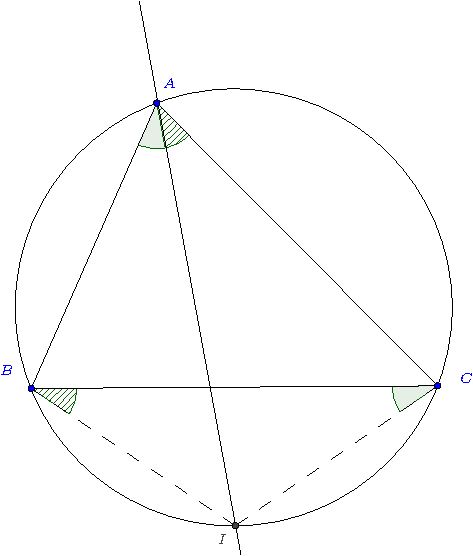
\includegraphics{../images/img007124-1}
\end{center}

Pour montrer que $BCI$ est isocèle en $I$, il suffit de montrer que $(BC,BI) = (CI,CB)$. Or, on a 
\begin{align*}
(BC,BI) &= (AC,AI) \text{ car $ABIC$ est inscriptible}\\
&= (AI,AB) \text{ car $(AI)$ est une bissectrice de $(AC)$ et $(AB)$}\\
&= (CI,CB) \text{ car $ABIC$ est inscriptible.}
\end{align*}

On remarque qu'en rédigeant avec des angles de droites, on n'a pas eu besoin (ni en fait la possibilité) de préciser si la bissectrice était intérieure ou extérieure, ce qui implique que la preuve sera la même pour $J$. Traçons juste une figure pour visualiser la deuxième situation.


\begin{center}
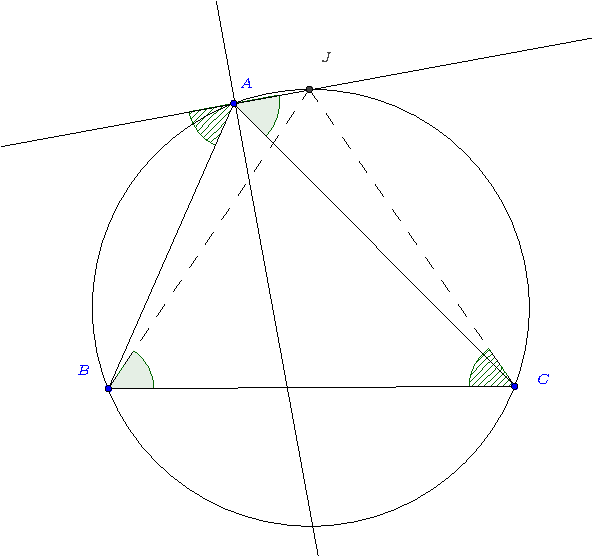
\includegraphics{../images/img007124-2}
\end{center}
}
}
